% ============================================================
%  RAPPORT DE STAGE — ZAKARIA LEMCHAOURI
%  OFPPT CMC Rabat — Wave Inc., Témara
%  Application : WAVE — Gestion Clients & Licences
% ============================================================

\documentclass[12pt, a4paper]{report}

% ---- Encodage & langue ----
\usepackage[utf8]{inputenc}
\usepackage[T1]{fontenc}
\usepackage[french, provide=*]{babel}
\usepackage{charter}

% ---- Mise en page ----
\usepackage[
  top=3cm, bottom=2.5cm,
  left=3cm,  right=2.5cm
]{geometry}
\usepackage{setspace}
\onehalfspacing

% ---- Couleurs & graphiques ----
\usepackage[dvipsnames, table]{xcolor}
\usepackage{graphicx}
\usepackage{tikz}
\usetikzlibrary{positioning, shapes.geometric, arrows.meta}

% Palette Wave
\definecolor{WaveBlue}{HTML}{1A73E8}
\definecolor{WaveDark}{HTML}{0D1B2A}
\definecolor{WaveAccent}{HTML}{00BFA5}
\definecolor{WaveGray}{HTML}{F5F7FA}
\definecolor{WaveBorder}{HTML}{E0E6ED}
\definecolor{HeaderBg}{HTML}{0D1B2A}

% ---- Typographie ----
\usepackage{microtype}

% ---- En-têtes & pieds de page avec logos ----
\usepackage{fancyhdr}
\usepackage{calc}
\pagestyle{fancy}
\fancyhf{}

% Header : logo OFPPT à gauche, logo CMC à droite
\fancyhead[L]{%
  \raisebox{-0.3\height}{
\includegraphics[height=1.4cm]{logos/ofppt.png}}%
}
\fancyhead[C]{\small\color{WaveBlue}\textit{Rapport de Stage \textbullet{} Zakaria Lemchaouri}}
\fancyhead[R]{%
  \raisebox{-0.3\height}{
\includegraphics[height=1.4cm]{logos/cmc.png}}%
}
\fancyfoot[C]{\thepage}
\renewcommand{\headrulewidth}{0.4pt}
\setlength{\headheight}{1.4cm}

% ---- Titres de chapitres en NOIR ----
\usepackage{titlesec}
\titleformat{\chapter}[hang]
  {\normalfont\huge\bfseries\color{black}}
  {CHAPITRE \thechapter.}
  {12pt}
  {\huge\bfseries\color{black}}[\vspace{4pt}\color{WaveBlue}\titlerule]
\titlespacing*{\chapter}{0pt}{10pt}{30pt}

\titleformat{\section}
  {\normalfont\Large\bfseries\color{black}}
  {\thesection}{1em}{}[\color{WaveBlue}\titlerule]
\titlespacing{\section}{0pt}{18pt}{8pt}

\titleformat{\subsection}
  {\normalfont\large\bfseries\color{black}}
  {\thesubsection}{1em}{}
\titlespacing{\subsection}{0pt}{14pt}{6pt}

% ---- Tableaux ----
\usepackage{booktabs}
\usepackage{tabularx}
\usepackage{multirow}
\usepackage{array}
\usepackage{longtable}

% ---- Listes ----
\usepackage{enumitem}
\setlist[itemize]{noitemsep, topsep=4pt, leftmargin=1.5em}

% ---- Code source ----
\usepackage{listings}
\lstset{
  basicstyle=\small\ttfamily,
  backgroundcolor=\color{WaveGray},
  frame=single,
  rulecolor=\color{WaveBorder},
  breaklines=true,
  captionpos=b,
  showstringspaces=false,
  keywordstyle=\color{WaveBlue}\bfseries,
  commentstyle=\color{gray}\itshape,
  stringstyle=\color{WaveAccent},
}

% ---- Liens hypertexte ----
\usepackage[
  colorlinks=true,
  linkcolor=WaveBlue,
  urlcolor=WaveAccent,
  citecolor=WaveDark,
  pdftitle={Rapport de Stage - Zakaria Lemchaouri},
  pdfauthor={Zakaria Lemchaouri},
]{hyperref}

% ---- Table des matières ----
\usepackage{tocloft}
\renewcommand{\cfttoctitlefont}{\Huge\bfseries\color{black}}
\renewcommand{\cftloftitlefont}{\Huge\bfseries\color{black}}
\renewcommand{\cftlottitlefont}{\Huge\bfseries\color{black}}
\renewcommand{\cftchapfont}{\bfseries\color{WaveDark}}
\renewcommand{\cftsecfont}{\color{WaveDark}}
\renewcommand{\cftchapleader}{\cftdotfill{\cftdotsep}}

% ---- Divers ----
\usepackage{caption}
\captionsetup{font=small, labelfont={bf,color=WaveBlue}}
\usepackage{float}
\usepackage{emptypage}

% ============================================================
%  MACROS
% ============================================================
\newcommand{\wave}{\textbf{\color{WaveBlue}WAVE}}
\newcommand{\ofppt}{\textsc{OFPPT}}
\newcommand{\HRule}{\rule{\linewidth}{0.5pt}}

% ============================================================
%  DOCUMENT
% ============================================================
\begin{document}

\pagenumbering{gobble}

% ============================================================
%  PAGE DE GARDE
% ============================================================
\begin{titlepage}
\centering

\begin{tikzpicture}[remember picture, overlay]
  \fill[WaveDark] (current page.north west)
    rectangle ([yshift=-3.2cm]current page.north east);
  \fill[WaveBlue] ([yshift=-3.2cm]current page.north west)
    rectangle ([yshift=-3.5cm]current page.north east);
\end{tikzpicture}

\vspace*{1.8cm}

\begin{minipage}{0.45\textwidth}
  \centering
  {\large\bfseries\color{WaveDark}OFPPT \textbullet{} CMC Rabat}
\end{minipage}
\hfill
\begin{minipage}{0.45\textwidth}
  \centering
  {\large\bfseries\color{WaveBlue}Wave Inc. \textbullet{} Témara}
\end{minipage}

\vspace{1.2cm}
\HRule\\[0.4cm]

{\huge\bfseries\color{WaveDark}Rapport de stage de fin de formation}\\[0.3cm]
{\large Présenté en vue de l'obtention du diplôme de}\\[0.5cm]
{\LARGE\bfseries\color{WaveBlue}TECHNICIEN SPÉCIALISÉ}\\[0.15cm]
{\LARGE\bfseries\color{WaveBlue}EN DÉVELOPPEMENT DIGITAL}\\[0.4cm]
\HRule

\vspace{0.8cm}

\fcolorbox{WaveBlue}{WaveGray}{%
\begin{minipage}{0.82\textwidth}
  \centering\vspace{0.5cm}
  {\LARGE\bfseries\color{WaveBlue}WAVE}\\[0.2cm]
  {\large\bfseries\color{WaveDark}Plateforme de Gestion Clients et Licences}\\[0.2cm]
  {\normalsize Développement d'une application web full-stack\\
  pour la gestion commerciale et la gestion des licences logicielles}
  \vspace{0.5cm}
\end{minipage}%
}

\vspace{0.8cm}

{\large\itshape Réalisé par}\\[0.3cm]
{\LARGE\bfseries\color{WaveDark}M.\ LEMCHAOURI Zakaria}

\vspace{0.8cm}

\begin{tabular}{@{}ll@{}}
  \textbf{Organisme :}                 & Wave Inc., Témara, Maroc \\[4pt]
  \textbf{Encadrant professionnel :}   & M. Mohamed Aherdane \\[4pt]
  \textbf{Encadrante pédagogique :}    & Mme. Ourrahte Malak \\
\end{tabular}

\vfill

{\normalsize Soutenu le \underline{\hspace{2cm}} /\underline{\hspace{2cm}} / 2026 \quad Devant le jury :}\\[0.5cm]
\begin{tabular}{@{}lll@{}}
  M./Mme.\ \underline{\hspace{3.8cm}} & Formateur Développement Digital & \textbf{Président du jury}\\[4pt]
  M./Mme.\ \underline{\hspace{3.8cm}} & Formateur Développement Digital & \textbf{Examinateur}\\
\end{tabular}

\begin{tikzpicture}[remember picture, overlay]
  \fill[WaveBlue] ([yshift=1.2cm]current page.south west)
    rectangle ([yshift=1.5cm]current page.south east);
  \fill[WaveDark] (current page.south west)
    rectangle ([yshift=1.2cm]current page.south east);
\end{tikzpicture}

\end{titlepage}

\cleardoublepage

% ============================================================
%  DÉDICACES
% ============================================================
\chapter*{Dédicaces}
\addcontentsline{toc}{chapter}{Dédicaces}

\vspace*{1cm}

\begin{flushright}
{\Large\itshape À ceux qui ont toujours cru en moi\ldots}
\end{flushright}

\vspace{1.5cm}

\begin{center}
\itshape

\textbf{À mes parents,}

\vspace{0.5cm}

Il y a des soutiens qu'on ne mesure qu'avec le recul. Chaque sacrifice
que vous avez consenti, chaque mot d'encouragement glissé au bon moment,
chaque regard plein de confiance ont été le carburant silencieux de ce
parcours. Ce diplôme porte votre nom autant que le mien, et je vous en
suis infiniment reconnaissant.

\vspace{1.2cm}

\textbf{À ma famille,}

\vspace{0.5cm}

Votre présence chaleureuse et votre soutien constant ont été un ancrage
précieux, aussi bien dans les moments de doute que dans ceux de fierté.
Merci d'avoir toujours été là.

\vspace{1.2cm}

\textbf{À mes amis et camarades de promotion,}

\vspace{0.5cm}

Ces deux années n'auraient pas eu la même saveur sans vous. Les sessions
de travail tardives, les débats techniques qui s'enflammaient pour
un rien, les fous rires qui décompressaient les journées intenses :
tout cela a fait partie de la formation, au même titre que les cours.
Merci pour tout.

\vspace{1.2cm}

\textbf{À toutes les personnes qui croient que l'effort finit toujours par payer.}

\vspace{2cm}

\normalsize\textit{Avec toute ma gratitude et mon respect.}

\end{center}

\cleardoublepage

% ============================================================
%  REMERCIEMENTS
% ============================================================
\chapter*{Remerciements}
\addcontentsline{toc}{chapter}{Remerciements}

\vspace*{0.5cm}

Ce rapport marque la fin d'une période de formation dense et
particulièrement enrichissante. Avant d'en présenter le contenu, je
tiens à exprimer ma reconnaissance envers toutes les personnes qui ont
contribué, de près ou de loin, à sa réalisation.

\vspace{0.6cm}

Mes premiers remerciements vont naturellement à \textbf{Wave Inc.} pour
m'avoir accueilli au sein de son équipe dans les meilleures conditions.
Travailler au sein d'une agence digitale active sur des projets réels
m'a permis de confronter rapidement mes acquis théoriques à des
problématiques concrètes, et d'apprendre bien plus vite qu'aucun cours
n'aurait pu me l'offrir seul.

\vspace{0.6cm}

Je remercie tout particulièrement \textbf{M.~Mohamed Aherdane},
mon encadrant professionnel, pour sa disponibilité, la clarté de ses
conseils et la confiance qu'il m'a accordée dans mes choix techniques.
Ses retours m'ont systématiquement poussé à remettre en question mes
solutions et à produire un travail plus rigoureux. J'ai beaucoup appris
à son contact.

\vspace{0.6cm}

J'adresse également ma gratitude à \textbf{Mme.~Ourrahte Malak},
encadrante pédagogique à l'\ofppt{} CMC Rabat, pour son suivi attentif
tout au long de la formation et pour les repères méthodologiques qu'elle
a su transmettre avec bienveillance. Sa disponibilité a été un vrai
appui dans les moments de flottement.

\vspace{0.6cm}

Je remercie l'ensemble du corps formateur de l'\ofppt{} CMC Rabat pour
la qualité de l'enseignement dispensé et pour avoir su nous transmettre,
au-delà des compétences techniques, une vraie façon de penser le
développement logiciel de manière professionnelle.

\vspace{0.6cm}

Enfin, je remercie les membres du jury pour le temps qu'ils consacreront
à l'évaluation de ce travail.

\vspace{1.5cm}

\begin{flushright}
\itshape Zakaria Lemchaouri\\
%Rabat, juin 2026
\end{flushright}

\cleardoublepage

% ============================================================
%  TABLE DES MATIÈRES
% ============================================================
\pagenumbering{roman}
\setcounter{page}{1}
\tableofcontents
\cleardoublepage

% ============================================================
%  TABLE DES FIGURES
% ============================================================
\listoffigures
\addcontentsline{toc}{chapter}{Table des figures}
\cleardoublepage

% ============================================================
%  LISTE DES TABLEAUX
% ============================================================
\listoftables
\addcontentsline{toc}{chapter}{Liste des tableaux}
\cleardoublepage

% ============================================================
%  ACRONYMES
% ============================================================
\chapter*{Acronymes}
\addcontentsline{toc}{chapter}{Acronymes}

\vspace{0.5cm}

\begin{longtable}{@{}p{3cm}p{11.5cm}@{}}
\toprule
\textbf{Sigle} & \textbf{Signification} \\
\midrule
\endhead
\textbf{API}   & Application Programming Interface \\[3pt]
\textbf{REST}  & Representational State Transfer \\[3pt]
\textbf{RBAC}  & Role-Based Access Control \\[3pt]
\textbf{HTTP}  & HyperText Transfer Protocol \\[3pt]
\textbf{HTTPS} & HyperText Transfer Protocol Secure \\[3pt]
\textbf{HTML}  & HyperText Markup Language \\[3pt]
\textbf{CSS}   & Cascading Style Sheets \\[3pt]
\textbf{JS}    & JavaScript \\[3pt]
\textbf{JSX}   & JavaScript XML \\[3pt]
\textbf{PHP}   & Hypertext Preprocessor \\[3pt]
\textbf{SQL}   & Structured Query Language \\[3pt]
\textbf{CRUD}  & Create, Read, Update, Delete \\[3pt]
\textbf{JSON}  & JavaScript Object Notation \\[3pt]
\textbf{URL}   & Uniform Resource Locator \\[3pt]
\textbf{UI}    & User Interface \\[3pt]
\textbf{UX}    & User Experience \\[3pt]
\textbf{BD}    & Base de Données \\[3pt]
\textbf{SPA}   & Single Page Application \\[3pt]
\textbf{SMTP}  & Simple Mail Transfer Protocol \\[3pt]
\textbf{MVC}   & Modèle, Vue, Contrôleur \\[3pt]
\textbf{UML}   & Unified Modeling Language \\[3pt]
\textbf{CORS}  & Cross-Origin Resource Sharing \\[3pt]
\textbf{MVP}   & Minimum Viable Product \\[3pt]
\textbf{ORM}   & Object-Relational Mapping \\[3pt]
\textbf{MAD}   & Dirham Marocain \\[3pt]
\textbf{CRM}   & Customer Relationship Management \\[3pt]
\textbf{PDF}   & Portable Document Format \\[3pt]
\textbf{CSV}   & Comma-Separated Values \\[3pt]
\textbf{KPI}   & Key Performance Indicator \\[3pt]
\textbf{JWT}   & JSON Web Token \\[3pt]
\textbf{SDK}   & Software Development Kit \\[3pt]
\textbf{CI/CD} & Continuous Integration et Continuous Deployment \\[3pt]
\textbf{FK}    & Foreign Key (Clé étrangère) \\[3pt]
\textbf{PK}    & Primary Key (Clé primaire) \\[3pt]
\textbf{MRR}   & Monthly Recurring Revenue (Revenu mensuel récurrent) \\[3pt]
\textbf{OFPPT} & Office de la Formation Professionnelle et de la Promotion du Travail \\[3pt]
\textbf{CMC}   & Cité des Métiers et des Compétences \\[3pt]
\bottomrule
\end{longtable}

\cleardoublepage

% ============================================================
%  INTRODUCTION GÉNÉRALE
% ============================================================
\pagenumbering{arabic}
\setcounter{page}{1}

\chapter*{Introduction Générale}
\addcontentsline{toc}{chapter}{Introduction Générale}
\markboth{Introduction Générale}{Introduction Générale}

\vspace{0.5cm}

La transformation numérique occupe aujourd'hui une place centrale dans la
stratégie des entreprises marocaines, tous secteurs confondus. Face à une
concurrence de plus en plus vive et à des clients dont les attentes ne
cessent de croître, les agences digitales et les éditeurs de logiciels
ont besoin d'outils internes solides pour piloter leur activité, gérer
leurs portefeuilles clients et assurer un suivi fiable de leurs licences
logicielles. Dans la réalité, beaucoup de structures de taille
intermédiaire s'appuient encore sur des solutions fragmentées :
tableurs, échanges par email, fichiers partagés en vrac. Le résultat,
c'est des pertes d'information régulières, des doublons qui s'accumulent
et une visibilité insuffisante sur la santé réelle de l'activité.

\vspace{0.6cm}

C'est précisément ce constat qui est à l'origine de ce stage, réalisé au
sein de \textbf{Wave Inc.}, une agence digitale établie à Témara. L'entreprise
accompagne des clients marocains dans leur transition numérique en leur
proposant des solutions web sur mesure ainsi que des produits SaaS. Avant
le lancement de ce projet, la gestion des clients, des paiements, des
licences et des contrats reposait en grande partie sur des processus
manuels peu coordonnés, ce qui rendait le suivi quotidien laborieux et
compliquait toute lecture globale de la performance commerciale.

\vspace{0.6cm}

La mission confiée consistait donc à concevoir et développer \wave{}, une
application web full-stack dédiée à la gestion commerciale et à la gestion
de licences. L'idée centrale était simple : regrouper dans une seule
plateforme cohérente l'ensemble des opérations du back-office, à savoir
la gestion des clients, des paiements, des contrats, des factures et du
pipeline commercial. En parallèle, les clients devaient disposer d'un
espace personnel pour consulter leurs licences actives, leurs factures,
leurs contrats, et passer des commandes directement en ligne via une
intégration \textbf{PayPal}.

\vspace{0.6cm}

L'application a été conçue selon une architecture \textbf{API-first},
avec un backend en \textbf{Laravel~13} exposant une API REST sécurisée
grâce à \textbf{Laravel Sanctum}, et un frontend en \textbf{React~19}
construit avec \textbf{Vite}. Cette séparation claire entre les deux
couches facilite la maintenance du code, améliore la scalabilité et
offre une expérience utilisateur fluide sous forme de Single Page
Application. Le système gère trois profils distincts : \textbf{admin},
\textbf{manager} et \textbf{client}, dont les droits d'accès sont
contrôlés de façon granulaire via un middleware de rôle côté serveur
et un système de routes protégées côté client.

\vspace{0.6cm}

Parmi les fonctionnalités les plus notables, on peut citer la génération
automatique de factures numérotées au format \texttt{FAC-YYYY-NNNN},
l'export de documents en PDF via \textbf{Laravel DomPDF}, un système
de relances et d'alertes pour les contrats arrivant à expiration, un
journal d'audit basé sur \textbf{Spatie ActivityLog}, et un tableau
de bord analytique avec visualisation des revenus mensuels grâce à
\textbf{Chart.js}. Des tâches planifiées envoient par ailleurs des
emails automatiques aux clients dont les licences approchent de leur
terme ou qui accusent un retard de paiement.

\vspace{0.6cm}

Ce rapport retrace l'ensemble de la démarche suivie pour mener ce projet
à bien, en trois chapitres~:

\vspace{0.4cm}

\begin{itemize}
  \item \textbf{Chapitre 1 (Contexte Général du Projet) :} présentation
  de l'organisme d'accueil Wave Inc., analyse de la situation existante,
  identification des problèmes rencontrés et spécification des besoins
  fonctionnels et non fonctionnels de la solution.

  \item \textbf{Chapitre 2 (Analyse et Conception) :} modélisation du
  système à l'aide des outils UML (diagrammes de cas d'utilisation, de
  séquence et de classes), conception du schéma de base de données et
  définition de l'architecture technique retenue.

  \item \textbf{Chapitre 3 (Réalisation) :} présentation des choix
  technologiques justifiés, description des modules développés, aperçu
  des interfaces réalisées et bilan des fonctionnalités livrées.
\end{itemize}

\vspace{0.6cm}

À titre personnel, ce stage a représenté une expérience particulièrement
marquante. Au-delà des compétences techniques approfondies, que ce soit
en développement backend Laravel, en conception d'API REST, en intégration
de paiement en ligne, en automatisation par tâches planifiées ou en gestion
des permissions par rôle, c'est surtout la confrontation à un projet réel
mené de bout en bout qui aura été la vraie valeur ajoutée. Ce rapport
conclut deux années de formation en Développement Digital à l'\ofppt{}
CMC Rabat et constitue une première immersion concrète dans les exigences
du terrain.

% ============================================================
%  Les chapitres seront ajoutés ici :
%  \input{chapitre1}
 
 
% ============================================================

% ============================================================
%  CHAPITRE 1 : CONTEXTE GENERAL DU PROJET
% ============================================================
%\chapter{Contexte General du Projet}
\clearpage
\thispagestyle{empty} % Supprime le numéro et l'en-tête sur cette page

% Modification temporaire du style : ajoute un \clearpage APRÈS le titre
\titleformat{\chapter}[display]
  {\normalfont\bfseries\color{black}\centering}
  {\Large CHAPITRE \thechapter}
  {20pt}
  {\Huge}[\clearpage]

\titlespacing*{\chapter}{0pt}{150pt}{0pt} % Ajuste la hauteur pour le centrage vertical

\chapter{Contexte General du Projet}
\label{ch:contexte_general}

% Restauration du style d'origine pour que les chapitres suivants fonctionnent normalement
\titleformat{\chapter}[display]
  {\normalfont\bfseries\color{black}\centering}
  {\Large CHAPITRE \thechapter}
  {20pt}
  {\Huge}
\titlespacing*{\chapter}{0pt}{80pt}{40pt}

% ============================================================
\section{Introduction}
% ============================================================

Ce premier chapitre pose les bases du projet en presentant l'environnement
dans lequel il s'inscrit. On y trouve la description de l'organisme d'accueil,
l'analyse de la situation avant le projet, les problemes concrets qui ont motive
le developpement de \wave{}, ainsi que la specification detaillee des besoins
fonctionnels et non fonctionnels de la solution. L'objectif est de donner au
lecteur une vision claire du "pourquoi" avant d'aborder le "comment" dans les
chapitres suivants.

% ============================================================
\section{Presentation de l'organisme d'accueil}
% ============================================================

\subsection{Identite et historique}

Wave Inc. est une agence digitale a service complet, fondee le 26 mai 2015 au
Maroc. L'entreprise est enregistree sous forme juridique de Societe a
Responsabilite Limitee (SARL) avec un capital social de 500 000 DHS. Sa
gouvernance repose sur un dirigeant principal associe a trois co-associes.

Depuis sa creation, l'agence a connu plusieurs etapes de restructuration pour
accompagner sa croissance. Un premier transfert de siege social accompagne d'une
cession de parts sociales a eu lieu en novembre 2016, suivi d'une augmentation
de capital en mars 2021 et d'un second transfert de siege en juillet 2022, ce
qui temoigne d'une trajectoire de developpement continue depuis dix ans.

\subsection{Implantation geographique}

Bien que la communication institutionnelle de l'agence mette en avant un ancrage
strategique au coeur de Rabat, son etablissement principal est situe sur
l'Avenue Mohammed V a Temara, a une quinzaine de minutes de la capitale. Cette
localisation offre un double avantage : des couts d'exploitation immobiliere
mieux maitrises, tout en maintenant une proximite directe avec les grands
donneurs d'ordres institutionnels et les ministeres bases a Rabat.

Pour renforcer son positionnement a l'international et capter des contrats de
sous-traitance sur le marche europeen, Wave Inc. dispose egalement d'un bureau
de liaison commerciale en France, situe au Blanc Mesnil en region parisienne.

Le tableau \ref{tab:identite_wave} recapitule les principales donnees
administratives et de contact de l'agence.

\vspace{0.4cm}
\begin{table}[H]
\centering
\caption{Donnees d'identification de Wave Inc.}
\label{tab:identite_wave}
\begin{tabularx}{\textwidth}{@{}lX@{}}
\toprule
\textbf{Parametre} & \textbf{Donnee} \\
\midrule
Denomination sociale     & WAVE INC. SARL \\
Date de creation         & 26 mai 2015 \\
Forme juridique          & SARL -- Capital social : 500 000 DHS \\
Siege social             & 5, Lot Mohamed Et Jamila, 1er Etage, Temara \\
Etablissement principal  & 5, Avenue Mohammed V, 12000 Temara, Maroc \\
Bureau secondaire        & 10, Avenue de Rome, 93150 Le Blanc Mesnil, France \\
Horaires                 & Lundi au vendredi, 09h00 -- 18h00 \\
Telephone                & +212 (0) 537 612 736 / +212 (0) 809 893 112 \\
Email general            & contact@wave.ma \\
Email RH                 & rh@wave.ma \\
\bottomrule
\end{tabularx}
\end{table}

\subsection{Positionnement et services}

Wave Inc. se positionne comme un partenaire technologique de bout en bout pour
ses clients, en couvrant l'ensemble du cycle de vie d'un projet numerique. Cette
approche globale se distingue des agences specialisees sur un seul metier comme
le design ou le referencement.

Les services proposes couvrent le developpement web et mobile, la conception
d'interfaces utilisateur, l'integration de systemes via des API, le deploiement
et la maintenance d'applications, ainsi que l'accompagnement dans la
transformation digitale des entreprises.

Sur le plan technique, l'agence maitrise un ecosysteme technologique large et
coherent, detaille dans le tableau \ref{tab:stack_wave}.

\vspace{0.4cm}
\begin{table}[H]
\centering
\caption{Stack technologique de Wave Inc.}
\label{tab:stack_wave}
\begin{tabularx}{\textwidth}{@{}lX@{}}
\toprule
\textbf{Couche} & \textbf{Technologies utilisees} \\
\midrule
Frontend   & React JS, Vue.js, Angular, Nuxt.js, TypeScript \\
Backend    & Laravel, Symfony, CodeIgniter, CakePHP \\
Mobile     & React Native, Flutter, Ionic \\
CMS        & WordPress, Drupal, Prestashop, WooCommerce \\
APIs       & REST, SOAP, WebSockets \\
\bottomrule
\end{tabularx}
\end{table}

\subsection{Methodologie de travail}

La methodologie d'ingenierie appliquee par Wave Inc. s'inspire des frameworks
agiles. Les projets sont decoupes en cycles de developpement courts et iteratifs,
ce qui permet une mise en production progressive et un ajustement continu en
fonction des retours clients. Les problematiques de performance, de securite et
de referencement sont integrees des la phase de prototypage, plutot que traitees
tardivement comme de simples correctifs.

L'onboarding d'un nouveau projet suit trois jalons : une phase de proposition
avec estimation de l'effort sous 24 heures, une phase de cadrage technique avec
le client, puis un demarrage immediat apres signature du contrat.

Concernant les modeles contractuels, l'agence propose deux formules. Le forfait
global est utilise quand le perimetre fonctionnel est bien defini en amont,
avec un prix ferme et un pilotage entierement pris en charge par l'agence. Le
mode regie est prefere pour les projets de longue duree ou les besoins evoluent,
avec une equipe dediee dont la composition peut etre ajustee selon la charge.

\subsection{Quelques realisations notables}

La credibilite technique de Wave Inc. est illustree par des projets realises
pour des structures publiques et privees exigeantes.

L'agence a assure le developpement du site institutionnel officiel du Conseil
de la Concurrence du Royaume du Maroc, une autorite administrative independante
de rang constitutionnel. Ce type de projet impose des criteres stricts en
matiere d'accessibilite, de securite des donnees et de disponibilite de
l'infrastructure pour faire face aux pics de trafic lors de publications de
rapports sensibles.

Elle a egalement concu la plateforme numerique complete de 2S Africa Travel,
une agence de voyage haut de gamme agreee par le Ministere du Tourisme marocain.
La solution integre des modules de tarification dynamique, la gestion de flux de
reservations complexes et des connexions de paiement securisees avec des
operateurs comme Visa, Mastercard et Payzone.

Ces references attestent de la capacite de l'agence a livrer des solutions
logicielles robustes dans des contextes ou la fiabilite et la securite ne sont
pas negociables.

% ============================================================
\section{Cadre du projet}
% ============================================================

\subsection{Problematique}

Malgre son expertise technique et la qualite de ses realisations pour ses
clients, Wave Inc. n'avait pas consacre le meme niveau d'attention a ses propres
outils de gestion interne. La gestion du portefeuille clients, des licences
logicielles, des paiements et des contrats reposait sur des fichiers Excel et
Google Sheets mis a jour manuellement. Chaque information existait dans un
fichier different, sans lien entre les donnees, et sans aucun mecanisme
d'alerte automatique.

Cette situation engendrait plusieurs problemes concrets au quotidien. Un manager
ne savait pas, sans aller fouiller dans plusieurs fichiers, si un client avait
des licences sur le point d'expirer ou des paiements en retard. La creation
d'une facture necessitait de recopier manuellement les informations du client
depuis une feuille vers une autre. Il n'existait aucune trace structuree des
echanges commerciaux avec un client, aucun historique consolide des paiements
et aucune vision globale des performances mensuelles sans construire soi-meme
des tableaux recapitulatifs.

Plus l'activite grandissait, plus cette approche montrait ses limites. Le risque
d'erreur augmentait, le temps consacre aux taches administratives repetitives
s'alourdissait et la qualite du suivi client se degradait faute d'un outil
centralise.

\subsection{Analyse de l'existant}

Avant le developpement de \wave{}, le processus de gestion d'un client
ressemblait a ceci : les informations de base etaient saisies dans un fichier
Excel partage sur Google Drive, les paiements recus etaient notes dans un
autre onglet, les licences attribuees etaient listees dans un troisieme
tableau, et les rappels d'echeances de contrats etaient geres manuellement
par le manager concerne, souvent via des alertes dans son calendrier personnel.

Cette fragmentation posait plusieurs problemes identifies lors de l'analyse
de l'existant.

Premierement, il n'y avait aucune source de verite unique. Une information
modifiee dans un fichier n'etait pas automatiquement repercutee ailleurs,
ce qui generait des incoherences entre les donnees.

Deuxiemement, le suivi des licences etait entierement manuel. Aucun systeme
n'informait automatiquement l'equipe qu'une licence allait expirer dans une
semaine. C'est le manager qui devait consulter regulierement le fichier et
faire le calcul lui-meme.

Troisiemement, la generation de factures etait une operation longue et
repetitive. Il fallait ouvrir un modele Word ou Excel, recopier les
informations du client, calculer les montants, exporter en PDF et envoyer
par email. Aucune numerotation automatique n'existait, ce qui compliquait
la tracabilite des documents.

Quatriemement, les clients n'avaient aucune visibilite sur leur propre
situation. Ils ne pouvaient pas consulter leurs licences actives, leurs
factures ou leurs contrats sans contacter directement leur manager, ce qui
generait une charge supplementaire pour l'equipe.

Le tableau \ref{tab:analyse_existant} synthetise les principales limites
identifiees.

\vspace{0.4cm}
\begin{table}[H]
\centering
\caption{Analyse des limites du systeme existant}
\label{tab:analyse_existant}
\begin{tabularx}{\textwidth}{@{}lXl@{}}
\toprule
\textbf{Domaine} & \textbf{Probleme identifie} & \textbf{Impact} \\
\midrule
Donnees clients    & Informations dispersees dans plusieurs fichiers
                     sans synchronisation                          & Eleve \\[4pt]
Licences           & Aucune alerte automatique d'expiration        & Eleve \\[4pt]
Paiements          & Suivi manuel, pas d'historique consolide      & Moyen \\[4pt]
Facturation        & Generation manuelle, pas de numerotation auto & Moyen \\[4pt]
Contrats           & Pas d'alerte sur les echeances proches        & Eleve \\[4pt]
Espace client      & Aucun acces autonome pour les clients         & Moyen \\[4pt]
Reporting          & Aucun tableau de bord, construction manuelle  & Eleve \\[4pt]
Traçabilite        & Aucun journal des actions effectuees          & Moyen \\
\bottomrule
\end{tabularx}
\end{table}

\subsection{Solution proposee}

Face a ces constats, il a ete decide de developper \wave{}, une application
web full-stack centralisee qui regroupe l'ensemble de ces fonctionnalites dans
une interface unique et coherente.

La solution repond aux lacunes identifiees de la maniere suivante. Toutes les
donnees clients, paiements, licences, factures et contrats sont stockees dans
une base de donnees relationnelle unique, ce qui elimine les incoherences entre
fichiers. Des taches planifiees envoient automatiquement des emails d'alerte
aux clients dont les licences expirent dans sept jours ou qui accusent un
retard de paiement. La facturation est entierement automatisee avec une
numerotation sequentielle au format \texttt{FAC-YYYY-NNNN} et une generation
PDF en un clic. Les clients disposent d'un espace personnel ou ils peuvent
consulter leurs licences actives, leurs factures, leurs contrats et passer
de nouvelles commandes via PayPal. Un journal d'audit base sur Spatie
ActivityLog trace toutes les actions effectuees sur les ressources sensibles.
Un tableau de bord analytique avec visualisation graphique des revenus mensuels
permet aux managers de piloter leur activite sans construire manuellement
de tableaux recapitulatifs.

\subsection{Comparaison entre l'ancien systeme et WAVE}

Le tableau \ref{tab:comparaison} presente une synthese comparative entre
la situation avant le projet et les apports de la nouvelle plateforme.

\vspace{0.4cm}
\begin{table}[H]
\centering
\caption{Comparaison entre l'existant et la solution WAVE}
\label{tab:comparaison}
\begin{tabularx}{\textwidth}{@{}lXX@{}}
\toprule
\textbf{Fonctionnalite} & \textbf{Avant WAVE} & \textbf{Avec WAVE} \\
\midrule
Gestion clients    & Fichiers Excel separes  & Base de donnees centralisee \\[4pt]
Alertes licences   & Manuelle ou inexistante & Email automatique J-7 \\[4pt]
Generation facture & Copier-coller manuel    & PDF genere en un clic \\[4pt]
Numerotation       & Pas de standard         & FAC-YYYY-NNNN auto \\[4pt]
Espace client      & Inexistant              & Portail self-service \\[4pt]
Paiement en ligne  & Inexistant              & Commande via PayPal \\[4pt]
Tableau de bord    & Construction manuelle   & KPIs et graphiques temps reel \\[4pt]
Journal d'audit    & Inexistant              & Traçabilite complete (Spatie) \\[4pt]
Relances retards   & Email manuel du manager & Envoi automatique planifie \\[4pt]
Pipeline CRM       & Aucun                   & Module opportunites integre \\
\bottomrule
\end{tabularx}
\end{table}

% ============================================================
\section{Analyse et specification des besoins}
% ============================================================

La specification des besoins a ete conduite apres plusieurs echanges avec
l'encadrant professionnel M. Mohamed Aherdane, en analysant les processus
existants et en identifiant les points de friction les plus critiques. Les
besoins se repartissent en deux categories : fonctionnels, qui decrivent ce
que le systeme doit faire, et non fonctionnels, qui decrivent comment il doit
le faire.

\subsection{Besoins fonctionnels}

Les besoins fonctionnels ont ete organises par module, en distinguant les
fonctionnalites selon le role de l'utilisateur concerne.

\vspace{0.3cm}
\textbf{1. Authentification et gestion des roles}

\begin{itemize}
  \item Connexion securisee par email et mot de passe avec generation d'un
        token Bearer via Laravel Sanctum.
  \item Deconnexion avec invalidation immediate du token.
  \item Redirection automatique vers le tableau de bord correspondant au role
        apres connexion (admin, manager, client).
  \item Controle d'acces granulaire : chaque groupe de routes est protege par
        un middleware de verification du role.
  \item Provisionnement d'un compte utilisateur pour un client par le manager,
        sans que le client n'ait a s'inscrire lui-meme.
\end{itemize}

\vspace{0.3cm}
\textbf{2. Gestion des clients}

\begin{itemize}
  \item Creation, modification et suppression douce (soft delete) d'une fiche
        client avec les champs nom, email, telephone, societe, statut et notes.
  \item Recherche et filtrage de la liste des clients par nom, email ou statut
        (actif, en attente, en retard).
  \item Export de la liste complete des clients au format CSV.
  \item Consultation d'un journal d'audit par client, trace par Spatie
        ActivityLog, listant toutes les actions effectuees sur sa fiche.
\end{itemize}

\vspace{0.3cm}
\textbf{3. Gestion des paiements}

\begin{itemize}
  \item Enregistrement, modification et suppression douce de paiements, avec
        les informations montant (en MAD), date, reference et type
        (abonnement, licence, autre).
  \item Calcul automatique du total des paiements par client.
  \item Export du releve de paiements d'un client au format PDF via
        Laravel DomPDF.
\end{itemize}

\vspace{0.3cm}
\textbf{4. Gestion des licences}

\begin{itemize}
  \item Attribution d'une licence produit a un client avec date d'attribution
        et calcul automatique de la date d'expiration selon la duree du produit.
  \item Revocation d'une licence.
  \item Mise a jour automatique du statut de la licence : active, bientot
        expiree (a moins de 7 jours) ou expiree.
  \item Envoi d'un email de rappel automatique au client dont la licence expire
        dans exactement 7 jours.
\end{itemize}

\vspace{0.3cm}
\textbf{5. Gestion des factures}

\begin{itemize}
  \item Creation, modification et suppression douce de factures avec
        numerotation sequentielle automatique au format \texttt{FAC-YYYY-NNNN}.
  \item Telechargement individuel de chaque facture au format PDF.
  \item Liaison automatique entre une facture et le paiement correspondant.
\end{itemize}

\vspace{0.3cm}
\textbf{6. Gestion des contrats}

\begin{itemize}
  \item Creation, modification et suppression de contrats avec dates de debut
        et de fin, montant en MAD et manager responsable.
  \item Mise a jour automatique du statut du contrat (actif ou expire) selon
        la date du jour.
  \item Alerte sur les contrats expirant dans les prochains jours, accessible
        depuis le tableau de bord.
\end{itemize}

\vspace{0.3cm}
\textbf{7. Relances commerciales}

\begin{itemize}
  \item Creation et gestion de relances (follow-ups) associees a un client,
        avec note, date prevue et statut (faite ou non).
  \item Envoi automatique d'un email de rappel aux clients en statut "en retard"
        chaque lundi matin.
\end{itemize}

\vspace{0.3cm}
\textbf{8. Pipeline commercial}

\begin{itemize}
  \item Creation, modification et suppression d'opportunites commerciales avec
        titre, description, montant estime en MAD, statut et date de cloture
        prevue.
  \item Attribution d'une opportunite a un client et a un manager responsable.
\end{itemize}

\vspace{0.3cm}
\textbf{9. Tickets de support}

\begin{itemize}
  \item Soumission d'un ticket de support par le client depuis son espace
        personnel, avec sujet et message.
  \item Consultation et mise a jour du statut des tickets par le manager.
\end{itemize}

\vspace{0.3cm}
\textbf{10. Tableau de bord et statistiques}

\begin{itemize}
  \item Affichage des KPIs principaux : nombre total de clients, clients payes,
        clients en attente, clients en retard et revenu mensuel recurrent (MRR).
  \item Graphique des revenus par mois sur l'annee selectionnee.
  \item Alerte visuelle si des licences expirent dans les 7 prochains jours.
\end{itemize}

\vspace{0.3cm}
\textbf{11. Espace client}

\begin{itemize}
  \item Consultation des licences actives avec dates d'expiration.
  \item Consultation et telechargement des factures et contrats.
  \item Soumission et suivi de tickets de support.
  \item Consultation des notifications in-app et marquage comme lue.
  \item Acces a la boutique de produits et passation de commandes via PayPal.
  \item Export du releve personnel en PDF.
\end{itemize}

\vspace{0.3cm}
\textbf{12. Administration}

\begin{itemize}
  \item Creation, consultation et suppression de comptes managers par l'admin.
  \item Creation, modification, suppression et activation/desactivation de
        produits avec prix en MAD et duree de licence en jours.
  \item Definition et mise a jour des objectifs mensuels par manager.
\end{itemize}

\subsection{Besoins non fonctionnels}

Au-dela des fonctionnalites, la solution devait repondre a un ensemble
d'exigences de qualite.

\vspace{0.3cm}
\textbf{1. Securite}

Toutes les routes de l'API sont protegees par un token Bearer obligatoire.
Tout acces sans token valide est immediatement rejete avec une erreur HTTP 401.
Le middleware de role verifie, en plus de l'authentification, que l'utilisateur
connecte dispose bien des droits necessaires pour acceder a la ressource
demandee. Les mots de passe sont haches avec bcrypt. Un intercepteur Axios
cote frontend purge le token stocke en local et redirige vers la page de
connexion en cas de reponse 401 du serveur. Les politiques CORS sont
configurees pour n'accepter que les requetes provenant du frontend autorise.

\vspace{0.3cm}
\textbf{2. Performance}

Les emails sont envoyes de maniere asynchrone via le systeme de queues de
Laravel, de sorte que les actions de l'utilisateur ne soient jamais bloquees
par un envoi d'email. Les listes de clients et de paiements sont paginées
pour eviter de charger des volumes de donnees trop importants en une seule
requete.

\vspace{0.3cm}
\textbf{3. Ergonomie}

L'interface doit etre accessible sans formation particuliere. La navigation
doit etre intuitive et les actions importantes doivent etre accessibles en
un minimum de clics. Chaque role dispose de son propre layout avec uniquement
les menus qui le concernent, ce qui evite toute confusion entre les espaces.

\vspace{0.3cm}
\textbf{4. Fiabilite}

Toutes les entrees utilisateur sont validees cote serveur avant tout
traitement. Les suppressions de clients, paiements et factures sont
implementees en soft delete pour eviter toute perte accidentelle de donnees.
Les actions critiques comme la suppression d'un compte ou la modification
d'un statut sont protegees par des regles metier strictes.

\vspace{0.3cm}
\textbf{5. Maintenabilite}

Le backend est organise en modules independants par domaine fonctionnel.
Le frontend est structure en composants React reutilisables avec une separation
claire entre la logique d'etat et la presentation. Cette organisation facilite
l'ajout de nouveaux modules sans impacter les fonctionnalites existantes.

% ============================================================
\section{Gestion du projet}
% ============================================================

Le stage s'est deroule sur une duree de quatre semaines. La gestion du projet
a suivi une approche MVP (Minimum Viable Product) : developper d'abord les
fonctionnalites essentielles du systeme, a savoir l'authentification, la
gestion des clients et des paiements, avant d'enrichir progressivement la
plateforme avec les modules plus avances comme les notifications, le pipeline
commercial et l'espace client.

Le travail a ete realise en autonomie, avec des points reguliers avec
M. Mohamed Aherdane pour valider les choix techniques et les livrables de
chaque phase. Le code source a ete versionne sur GitHub via Git tout au long
du developpement, ce qui a permis de conserver un historique clair des
modifications et de revenir a des etats anterieurs si necessaire.

\subsection{Planification previsionnelle}

La figure \ref{fig:gantt} presente la repartition temporelle des differentes
phases du projet sous forme de diagramme de Gantt.

\vspace{0.4cm}
\begin{figure}[H]
\centering
\begin{tabular}{@{}p{5.5cm}cccc@{}}
\toprule
\textbf{Tache} & \textbf{S1} & \textbf{S2} & \textbf{S3} & \textbf{S4} \\
\midrule
Analyse des besoins et conception BD
  & \cellcolor{WaveBlue!60}\textcolor{white}{\textbf{---}}
  & & & \\[6pt]
Developpement backend (API REST)
  & & \cellcolor{WaveBlue!60}\textcolor{white}{\textbf{---}}
  & & \\[6pt]
Developpement frontend (React)
  & & & \cellcolor{WaveBlue!60}\textcolor{white}{\textbf{---}}
  & \\[6pt]
Tests, corrections et livraison
  & & & & \cellcolor{WaveBlue!60}\textcolor{white}{\textbf{---}} \\
\bottomrule
\end{tabular}
\caption{Diagramme de Gantt previsionnel du projet (4 semaines)}
\label{fig:gantt}
\end{figure}

La premiere semaine a ete consacree a l'analyse des besoins, a l'etude de
l'existant, a la conception de la base de donnees et au maquettage des
interfaces principales. La deuxieme semaine a porte sur le developpement du
backend : mise en place de l'API REST, authentification, gestion des clients,
paiements, licences, factures et contrats. La troisieme semaine a ete dediee
au frontend : construction des layouts par role, developpement des pages,
integration des appels API et mise en place de l'espace client. La quatrieme
semaine a ete reservee aux tests fonctionnels, corrections des bugs identifies
et finalisation des livraisons.

% ============================================================
\section{Conclusion}
% ============================================================

Ce premier chapitre a permis de poser le cadre du projet. La presentation de
Wave Inc. illustre une agence avec une expertise technique solide et des
references serieuses, mais dont les outils de gestion interne n'etaient pas
a la hauteur de cette expertise. L'analyse de l'existant a mis en evidence
des lacunes significatives : donnees dispersees, aucune automatisation des
alertes, generation de documents manuelle et aucune visibilite offerte aux
clients sur leur propre situation.

La solution \wave{} repond directement a ces problemes en centralisant
l'ensemble des processus dans une plateforme unique, structuree autour
d'une architecture API-first moderne et d'un systeme de roles permettant
a chaque utilisateur d'acceder uniquement a ce qui le concerne.

Le chapitre suivant sera consacre a la phase d'analyse et de conception,
avec la modelisation UML du systeme, la conception de la base de donnees
relationnelle et la definition de l'architecture technique retenue.


% ============================================================
%  CHAPITRE 2 : ANALYSE ET CONCEPTION
% ============================================================

\cleardoublepage
\thispagestyle{empty}

\titleformat{\chapter}[display]
  {\normalfont\bfseries\color{black}\centering}
  {\Large CHAPITRE \thechapter}
  {20pt}
  {\Huge}[\clearpage]
\titlespacing*{\chapter}{0pt}{150pt}{0pt}

\chapter{Analyse et Conception}
\label{ch:analyse_conception}

\titleformat{\chapter}[display]
  {\normalfont\bfseries\color{black}\centering}
  {\Large CHAPITRE \thechapter}
  {20pt}
  {\Huge}
\titlespacing*{\chapter}{0pt}{80pt}{40pt}

% ============================================================
\section{Introduction}
% ============================================================

Apres avoir pose le contexte du projet et specifie les besoins dans le
chapitre precedent, ce deuxieme chapitre aborde la phase d'analyse et de
conception. C'est une etape charniere : elle transforme des besoins exprimes
en langage naturel en une architecture logicielle precise et documentee,
sur laquelle le developpement pourra s'appuyer directement.

Nous presentons ici les outils et methodes de modelisation retenus, les
acteurs du systeme et leurs interactions a travers les diagrammes de cas
d'utilisation, les diagrammes de sequence illustrant les scenarios
principaux, ainsi que le diagramme de classes qui constitue la base
structurelle de la base de donnees de l'application.

% ============================================================
\section{Methodes et outils de modelisation}
% ============================================================

\subsection{Langage de modelisation UML}

UML (Unified Modeling Language) est un langage de modelisation graphique
standardise, largement adopte dans le domaine du genie logiciel. Il permet
de visualiser, specifier et documenter les differentes dimensions d'un
systeme, aussi bien sa structure statique que son comportement dynamique.

Dans le cadre de ce projet, UML a ete utilise pour produire trois types
de diagrammes complementaires :

\begin{itemize}
  \item Les \textbf{diagrammes de cas d'utilisation}, qui decrivent les
        interactions entre les acteurs et le systeme, et permettent de
        valider que l'ensemble des besoins fonctionnels est bien couvert.
  \item Les \textbf{diagrammes de sequence}, qui retracent le deroulement
        chronologique des echanges entre les composants du systeme lors
        des scenarios les plus importants.
  \item Le \textbf{diagramme de classes}, qui represente la structure des
        donnees, les entites du domaine et leurs relations, et sert de
        reference directe pour la conception de la base de donnees.
\end{itemize}

\subsection{Identification des acteurs}

Un acteur est toute entite externe qui interagit avec le systeme. Pour
l'application WAVE, quatre acteurs principaux ont ete identifies.

\textbf{L'Admin} est l'administrateur de la plateforme. Il dispose des
acces les plus etendus : il peut gerer les comptes managers, le catalogue
de produits, et definir les objectifs mensuels de chaque manager. Il herite
egalement de toutes les fonctionnalites du manager.

\textbf{Le Manager} est le commercial de l'agence. Il prend en charge le
suivi quotidien des clients : gestion des paiements, attribution des
licences, suivi des contrats et des relances, pilotage du pipeline
commercial et consultation des tickets de support.

\textbf{Le Client} est l'utilisateur final de l'espace client. Il
consulte ses licences actives, ses factures et ses contrats, soumet des
tickets de support et peut passer des commandes directement en ligne via
PayPal.

\textbf{Le Scheduler (Cron)} est un acteur systeme qui represente le
planificateur de taches de Laravel. Il declenche automatiquement des
traitements en arriere-plan : verification quotidienne des licences,
envoi d'emails de rappel et generation du rapport mensuel.

% ============================================================
\section{Diagrammes de cas d'utilisation}
% ============================================================

Les diagrammes de cas d'utilisation ont ete organises par acteur afin
de garder une lecture claire malgre le nombre important de fonctionnalites
couverts par la plateforme. Trois diagrammes ont ete produits, chacun
couvrant un perimetre fonctionnel distinct.

\subsection{Diagramme de cas d'utilisation -- Scheduler, Gestion Clients
            et Gestion Factures}

Le premier diagramme (Figure \ref{fig:dcu1}) regroupe les fonctionnalites
liees a la gestion des clients, a la facturation et aux automatisations
declenchees par le planificateur de taches.

Cote gestion des clients, le manager peut lister, rechercher, creer,
modifier et supprimer des fiches clients. Il peut egalement provisionner
un compte utilisateur pour un client et exporter la liste au format CSV.
La consultation de la fiche client sert de point d'entree pour acceder
aux autres modules : paiements, licences, contrats et relances.

Cote facturation, le manager cree des factures avec numerotation
automatique au format \texttt{FAC-YYYY-NNNN}, les modifie, les supprime
et peut telecharger chaque facture en PDF.

Le Scheduler prend en charge trois automatisations : il verifie et met
a jour le statut des licences chaque jour, envoie des rappels d'expiration
sept jours avant l'echeance, envoie des rappels de retard de paiement
chaque lundi, et genere un rapport mensuel envoye automatiquement aux admins.

\begin{figure}[H]
  \centering
  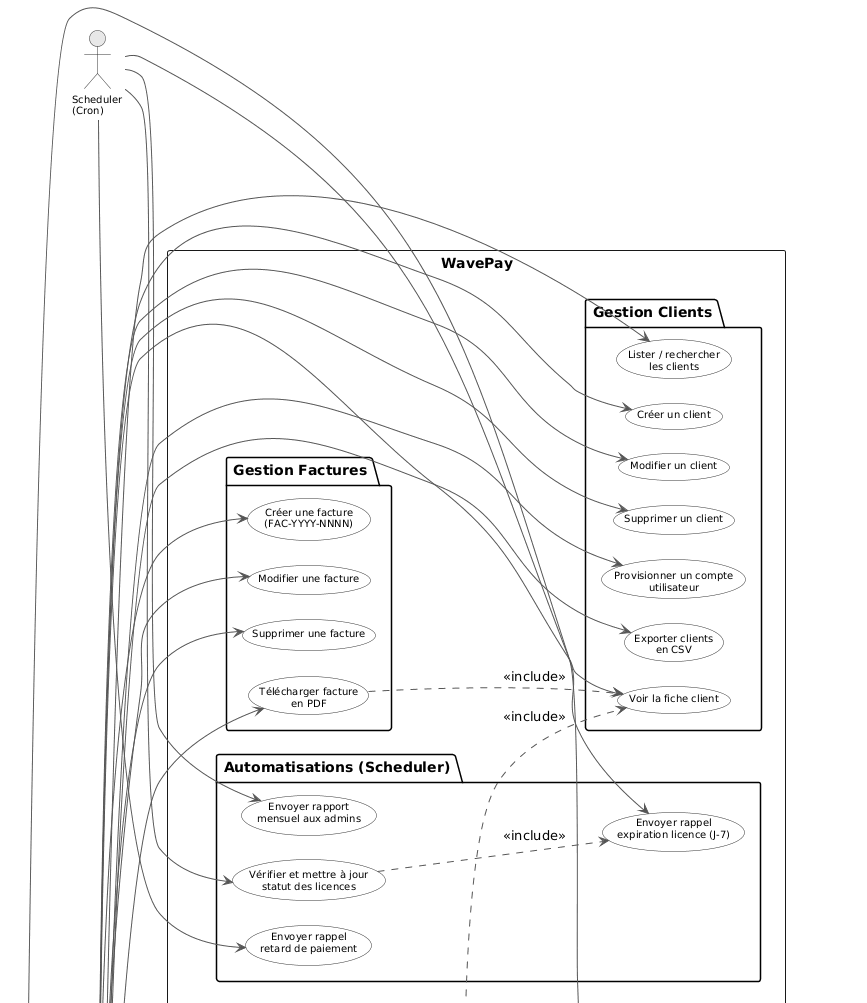
\includegraphics[width=0.82\textwidth]{diagrammes-casdutilisations/Diag-Cas-Utilisation-1.png}
  \caption{Diagramme de cas d'utilisation -- Scheduler, Clients et Factures}
  \label{fig:dcu1}
\end{figure}

\subsection{Diagramme de cas d'utilisation -- Manager}

Le deuxieme diagramme (Figure \ref{fig:dcu2}) est entierement dedie
au role Manager et couvre l'ensemble de son perimetre operationnel.

La \textbf{gestion des contrats} permet de creer, modifier et supprimer
des contrats, et de visualiser directement depuis le tableau de bord
les contrats qui expirent bientot.

Le module de \textbf{relances commerciales} (follow-ups) offre la
possibilite de creer, modifier et supprimer des relances associees a
un client, et de les marquer comme effectuees une fois realisees.

Le \textbf{pipeline commercial} centralise la gestion des opportunites
CRM : lister, creer, modifier et supprimer des opportunites avec leur
montant estime et leur date de cloture prevue.

La section \textbf{dashboard et reporting} donne acces au tableau de
bord avec KPIs et graphique des revenus mensuels, ainsi qu'au journal
d'activite (audit log Spatie) par client.

Enfin, la \textbf{gestion des paiements} couvre l'enregistrement, la
modification, la suppression et l'export en PDF du releve de paiements,
tandis que la \textbf{gestion des licences} permet d'attribuer, de
revoquer et de consulter les licences d'un client.

\begin{figure}[H]
  \centering
  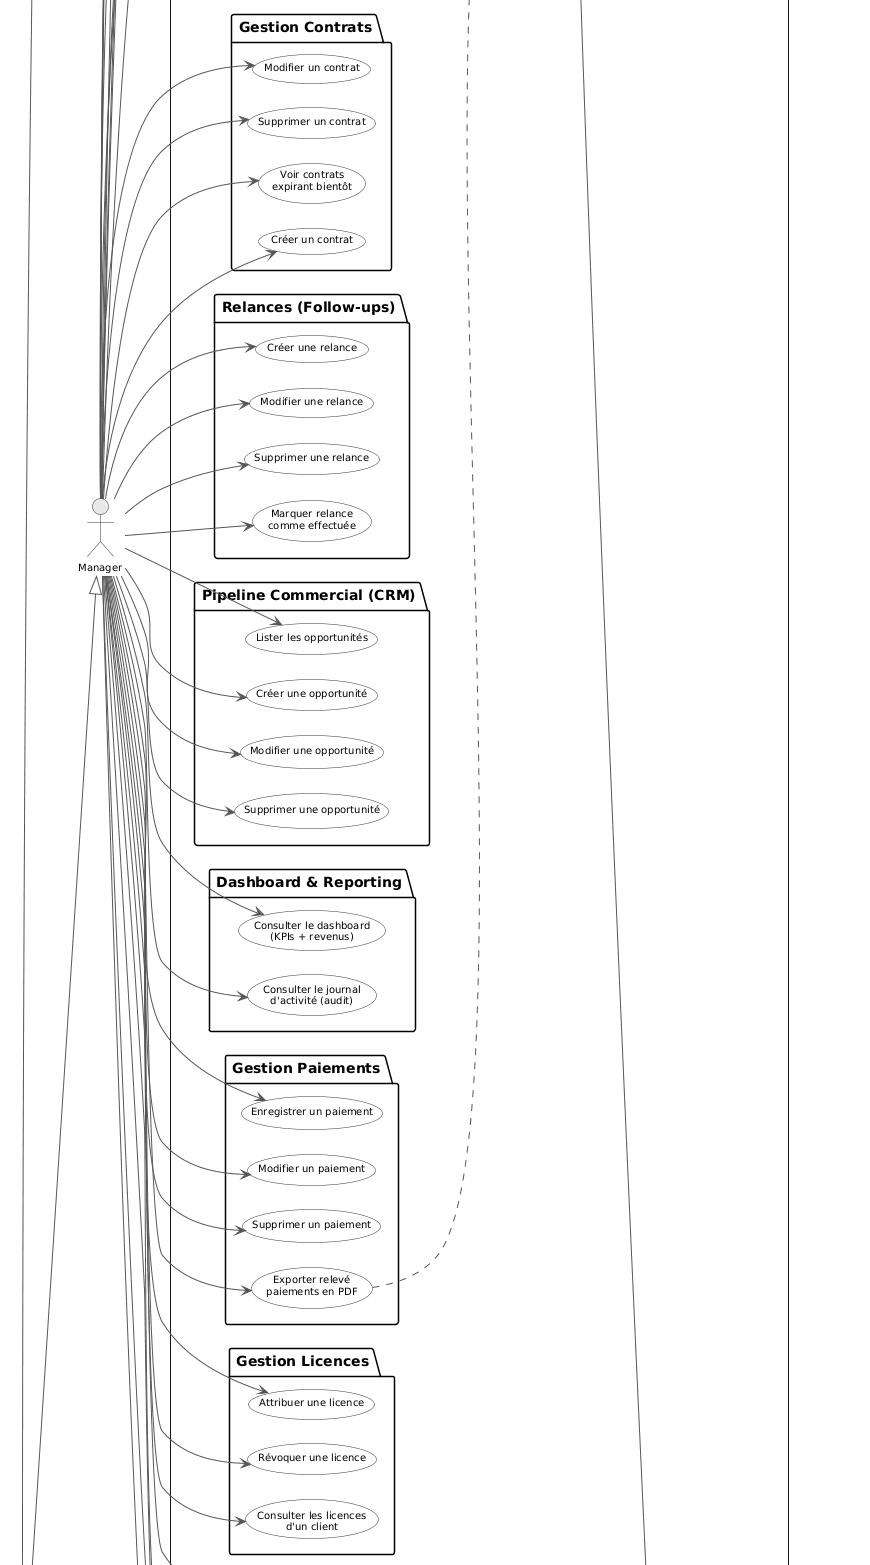
\includegraphics[width=0.72\textwidth]{diagrammes-casdutilisations/Diag-Cas-Utilisation-2.png}
  \caption{Diagramme de cas d'utilisation -- Manager}
  \label{fig:dcu2}
\end{figure}

\subsection{Diagramme de cas d'utilisation -- Admin et Client}

Le troisieme diagramme (Figure \ref{fig:dcu3}) regroupe les cas
d'utilisation specifiques a l'Admin et au Client.

Du cote \textbf{Admin}, le module d'authentification est commun a tous
les roles (connexion, deconnexion, consultation du profil via
\texttt{/me}). Le module de gestion admin lui permet de gerer les
managers en CRUD complet, de gerer le catalogue produits, d'activer
ou desactiver un produit et de definir les objectifs mensuels de chaque
manager. Il partage egalement l'acces aux tickets de support en vue
manager.

Du cote \textbf{Client}, l'espace personnel lui donne acces a son profil
et a ses licences actives, a ses factures avec telechargement PDF, a ses
contrats et a ses notifications in-app avec possibilite de les marquer
comme lues. Il peut exporter son releve personnel en PDF. Le module
boutique lui permet de parcourir le catalogue de produits actifs et de
passer une commande, ce qui inclut la redirection vers PayPal et la
confirmation du paiement via l'API PayPal SDK.

\begin{figure}[H]
  \centering
  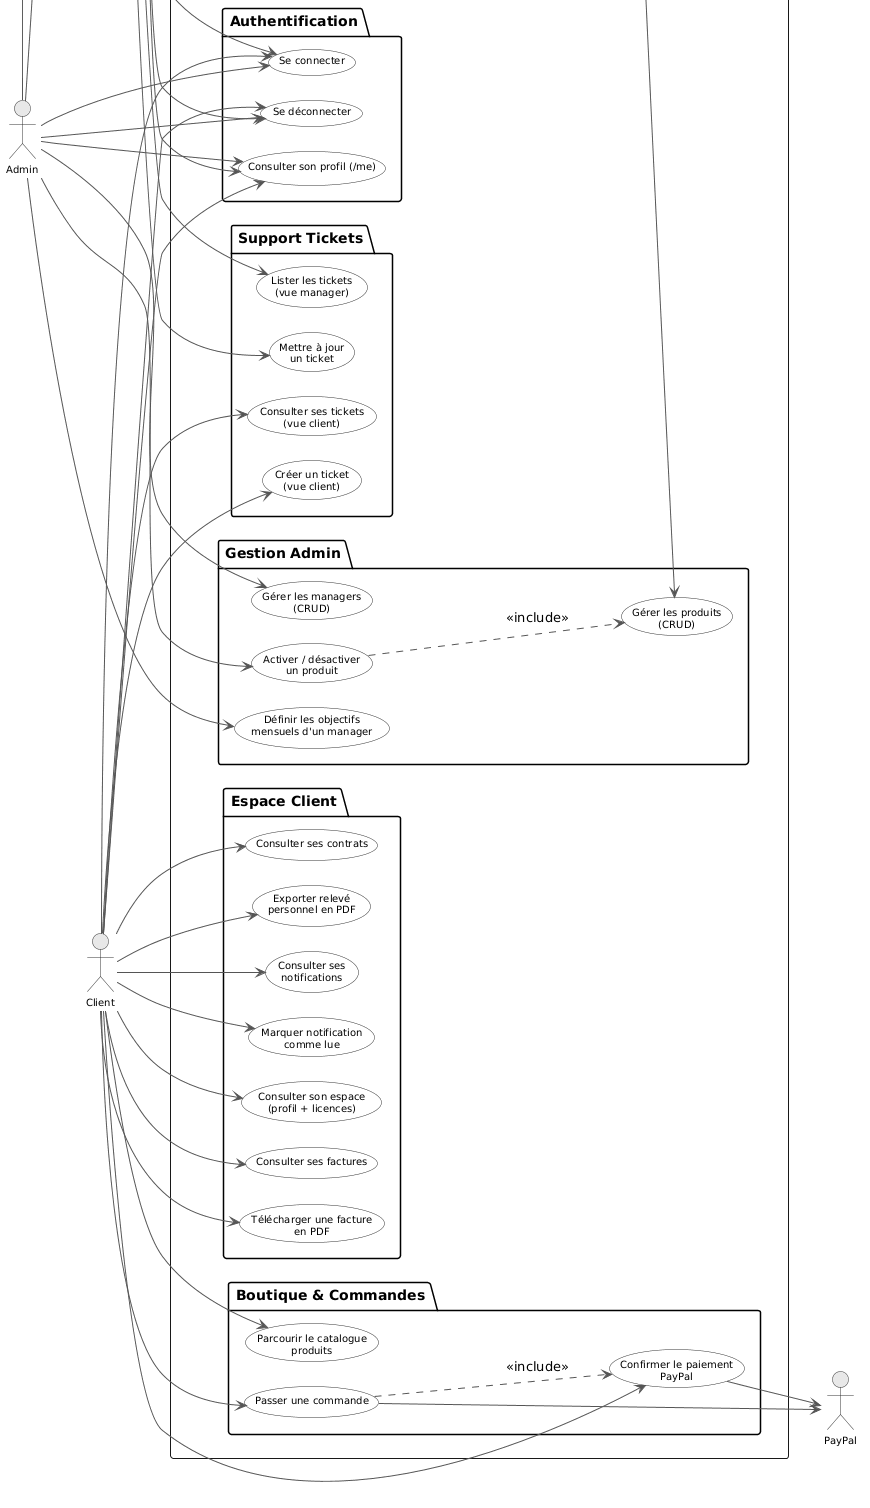
\includegraphics[width=0.82\textwidth]{diagrammes-casdutilisations/Diag-Cas-Utilisation-3.png}
  \caption{Diagramme de cas d'utilisation -- Admin et Client}
  \label{fig:dcu3}
\end{figure}

% ============================================================
\section{Diagrammes de sequence}
% ============================================================

Les diagrammes de sequence permettent de representer dans l'ordre
chronologique les echanges entre les differents composants du systeme
pour un scenario donne. Trois scenarios ont ete selectionnes parmi les
plus representatifs et les plus complexes de l'application.

\subsection{Sequence 1 -- Authentification et redirection par role}

Ce premier diagramme de sequence (Figure \ref{fig:seq1}) couvre deux
scenarios etroitement lies : la connexion d'un utilisateur et l'acces
a une route protegee.

Lors de la connexion, l'utilisateur saisit son email et son mot de passe
dans le formulaire React. Le frontend envoie une requete POST vers
\texttt{/api/v1/login}. Le backend interroge la base de donnees pour
verifier l'existence du compte et la validite du mot de passe. En cas
d'echec, une reponse 401 est retournee avec un message d'erreur affiche
cote client. Si les identifiants sont corrects, un token Sanctum est genere
et stocke dans la table \texttt{personal\_access\_tokens}. Le backend
retourne ce token accompagne des informations de l'utilisateur (id, nom,
role). Le frontend stocke le token dans le \texttt{localStorage} sous
la cle \texttt{wave\_token}, puis redirige automatiquement selon le
role : vers \texttt{/admin/dashboard} pour un admin, vers
\texttt{/manager/dashboard} pour un manager, ou vers \texttt{/client}
pour un client.

Lorsque l'utilisateur navigue vers une route protegee, le frontend joint
automatiquement le token dans l'en-tete HTTP \texttt{Authorization: Bearer}.
Le middleware Sanctum verifie la validite du token dans la table
\texttt{personal\_access\_tokens}. Si le token est invalide ou expire,
le backend retourne un 401, l'intercepteur Axios purge le \texttt{localStorage}
et redirige vers la page de connexion. Si le token est valide, l'utilisateur
est injecte dans la requete et l'acces est accorde.

\begin{figure}[H]
  \centering
  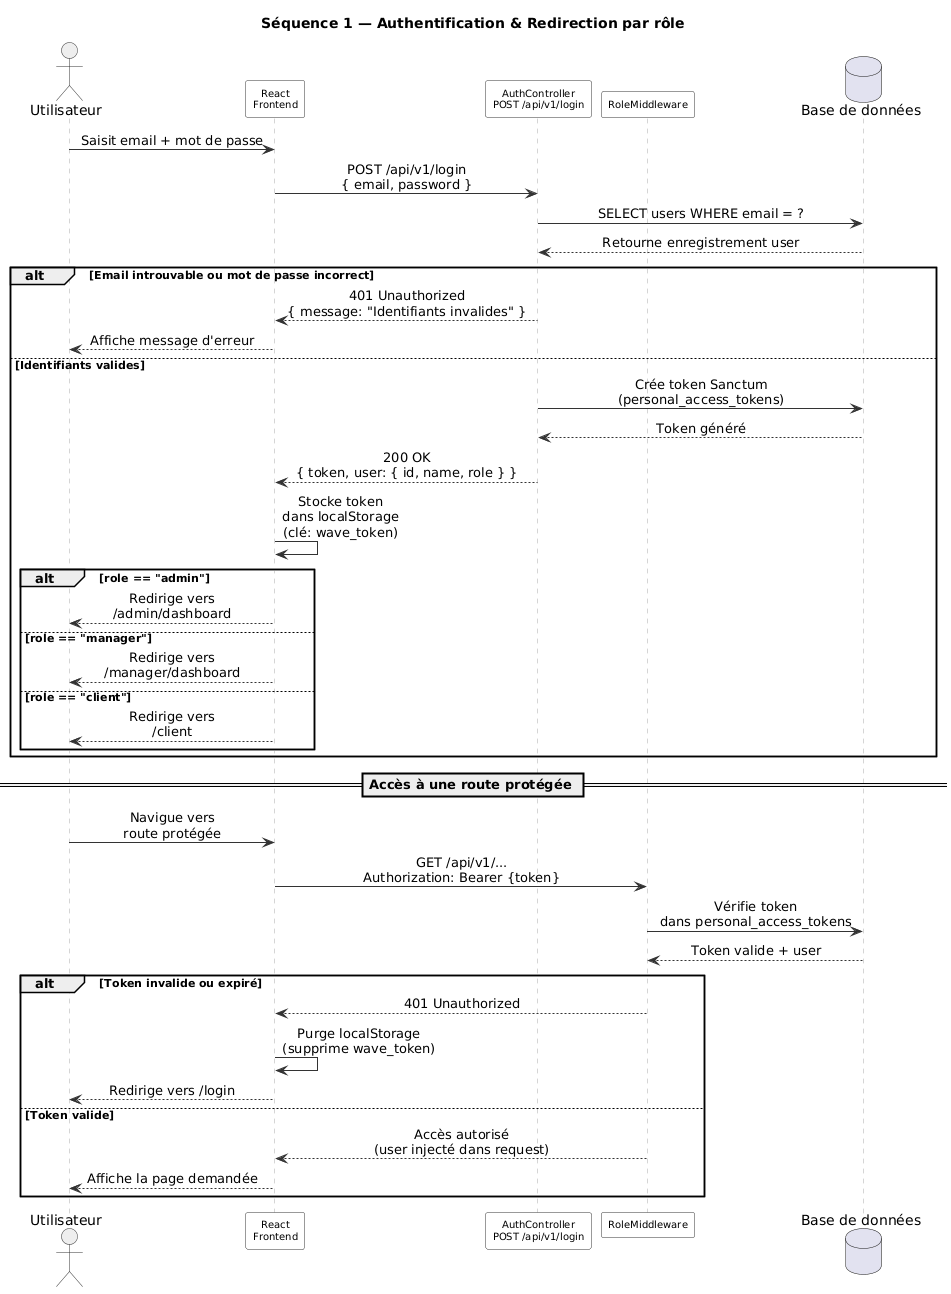
\includegraphics[width=\textwidth]{diagrammes-Sequances/authentification.png}
  \caption{Diagramme de sequence -- Authentification et redirection par role}
  \label{fig:seq1}
\end{figure}

\subsection{Sequence 2 -- Commande et paiement PayPal}

Le deuxieme diagramme de sequence (Figure \ref{fig:seq2}) retrace le
flux complet d'une commande depuis la boutique client jusqu'a l'attribution
automatique de la licence apres paiement confirme.

Le client parcourt le catalogue en appellant \texttt{GET /api/v1/client/shop},
qui retourne les produits dont le champ \texttt{is\_active} est vrai.
Quand il clique sur "Commander", le frontend envoie une requete POST vers
\texttt{/api/v1/client/shop/orders} avec l'identifiant du produit. Le
backend verifie que le produit est actif, recupere son prix, puis cree
un ordre PayPal via le SDK \texttt{srmklive/paypal} avec le montant en
MAD. L'identifiant et l'URL d'approbation PayPal sont retournes. Une
commande est inseree en base avec le statut \texttt{pending} et
l'identifiant PayPal. Le frontend redirige le client vers la page de
paiement PayPal via l'URL d'approbation.

Apres validation du paiement sur PayPal, le client est redirige vers
l'application. Le frontend envoie une requete POST vers
\texttt{/api/v1/client/shop/orders/\{order\_id\}/capture}. Le backend
recupere la commande, appelle \texttt{captureOrder} sur le SDK PayPal
avec l'identifiant PayPal. Si le paiement est refuse, le statut de la
commande est mis a \texttt{cancelled} et une erreur 402 est retournee.
Si la capture est confirmee, le backend met le statut a
\texttt{completed}, cree un enregistrement de paiement avec type
\texttt{license}, puis insere une entree dans la table pivot
\texttt{client\_license} avec les dates d'attribution et d'expiration
calculees automatiquement selon la duree du produit. Une reponse 200
confirme la commande et le frontend affiche les details de la licence
nouvellement activee.

\begin{figure}[H]
  \centering
  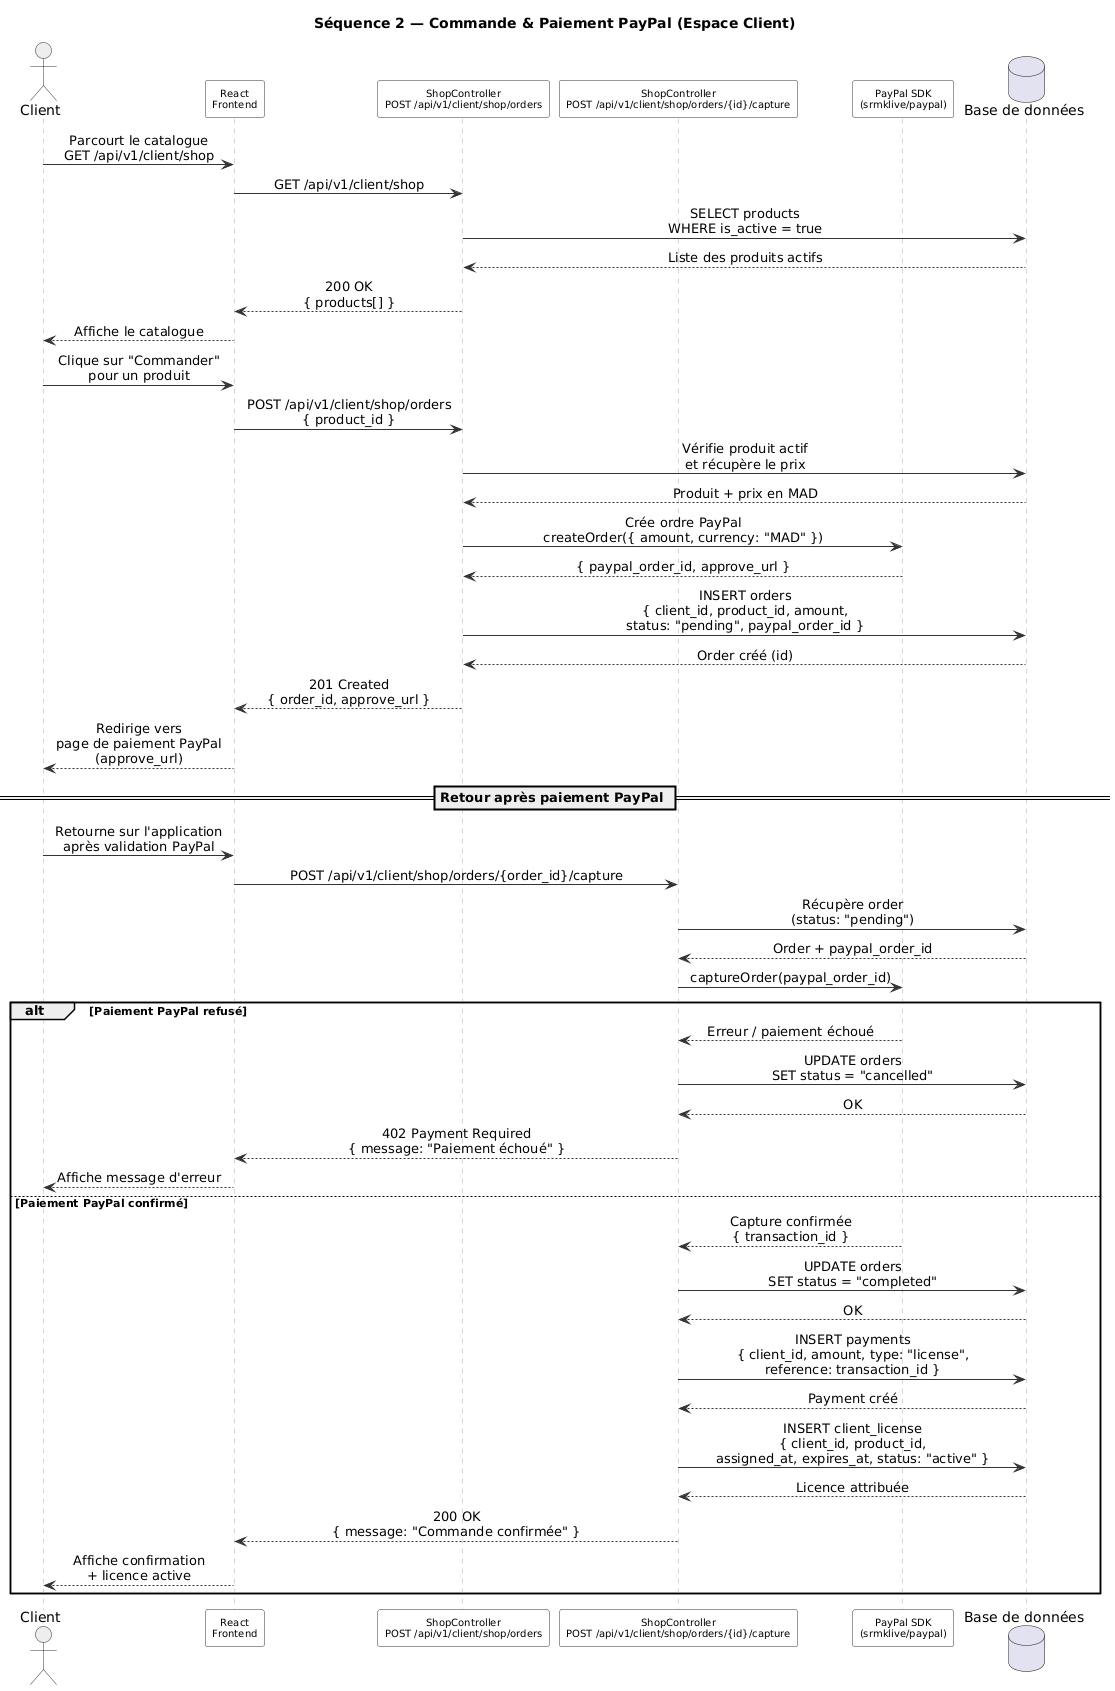
\includegraphics[width=\textwidth]{diagrammes-Sequances/paiment.png}
  \caption{Diagramme de sequence -- Commande et paiement PayPal}
  \label{fig:seq2}
\end{figure}

\subsection{Sequence 3 -- Verification automatique des licences}

Le troisieme diagramme de sequence (Figure \ref{fig:seq3}) illustre le
fonctionnement du systeme d'automatisation base sur le planificateur
de taches Laravel. Ce scenario ne fait intervenir aucune action manuelle
de la part d'un utilisateur : tout est declenche automatiquement.

Chaque jour a 08h00, le Scheduler dispatch le job \texttt{CheckLicenseExpiry}.
Ce job interroge la base pour recuperer toutes les licences dont la date
d'expiration est inferieure ou egale a la date du jour. Pour chacune d'elles,
il met a jour le statut a \texttt{expired}. Il effectue ensuite une seconde
requete pour identifier les licences dont l'expiration se situe entre
maintenant et dans sept jours. Pour chacune, il met le statut a
\texttt{expiring\_soon} et dispatch la notification
\texttt{LicenseExpiringNotification}. Cette notification est envoyee via
deux canaux en parallele : le canal \texttt{database}, qui insere une entree
dans la table \texttt{notifications} consultable depuis l'espace client,
et le canal \texttt{mail}, qui envoie un email via Laravel Mailer avec un
lien vers la boutique pour renouveler la licence.

Toujours a 08h00, le Scheduler dispatch le job
\texttt{SendLicenseExpiryReminder}. Celui-ci interroge la base pour trouver
les licences dont la date d'expiration correspond exactement a aujourd'hui
plus sept jours et dont le statut est \texttt{expiring\_soon}. Pour chaque
client concerne, il envoie individuellement un email de rappel avec un
lien vers la boutique.

Enfin, quand le client consulte ses notifications via
\texttt{GET /api/v1/client/notifications}, il recoit la liste des
notifications lues et non lues. Il peut ensuite marquer une notification
comme lue via \texttt{PATCH /api/v1/client/notifications/\{id\}/read},
ce qui retourne un 200 confirmant la mise a jour.

\begin{figure}[H]
  \centering
  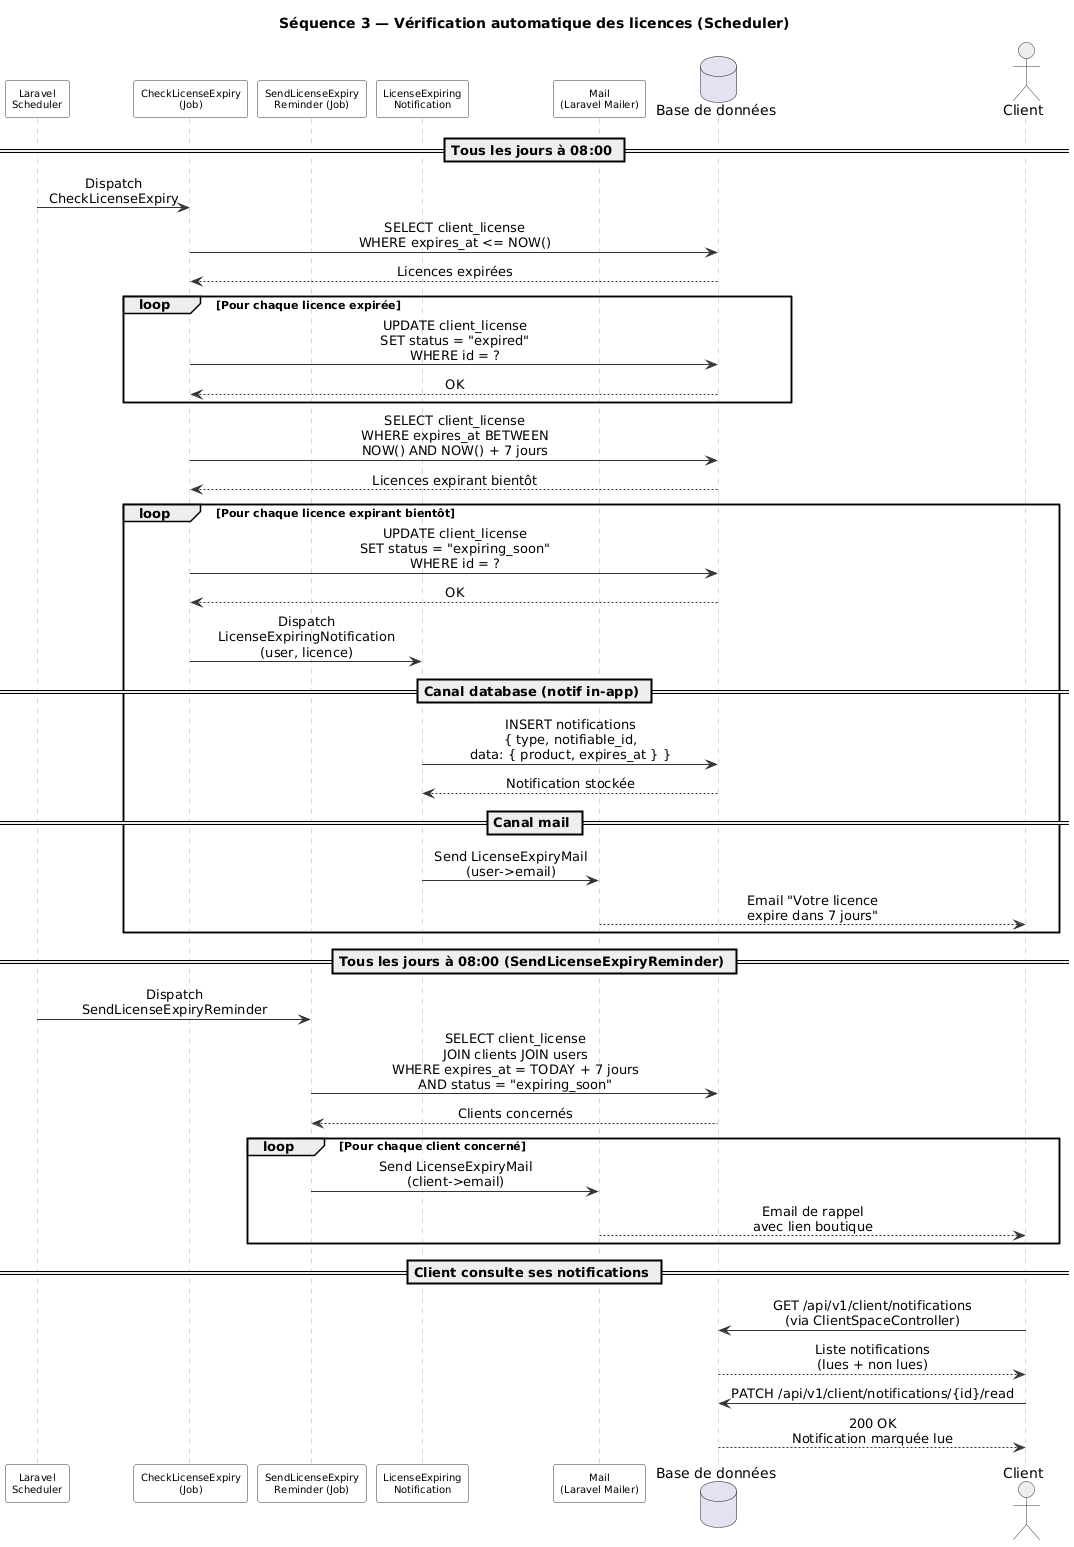
\includegraphics[width=\textwidth]{diagrammes-Sequances/verif-automatique des licences.png}
  \caption{Diagramme de sequence -- Verification automatique des licences}
  \label{fig:seq3}
\end{figure}

% ============================================================
\section{Diagramme de classes}
% ============================================================

Le diagramme de classes (Figure \ref{fig:classes}) represente la structure
statique du systeme. Il decrit les entites du domaine, leurs attributs,
leurs methodes et les relations qui les unissent. Il constitue la reference
directe pour la conception du schema de base de donnees.

\begin{figure}[H]
  \centering
  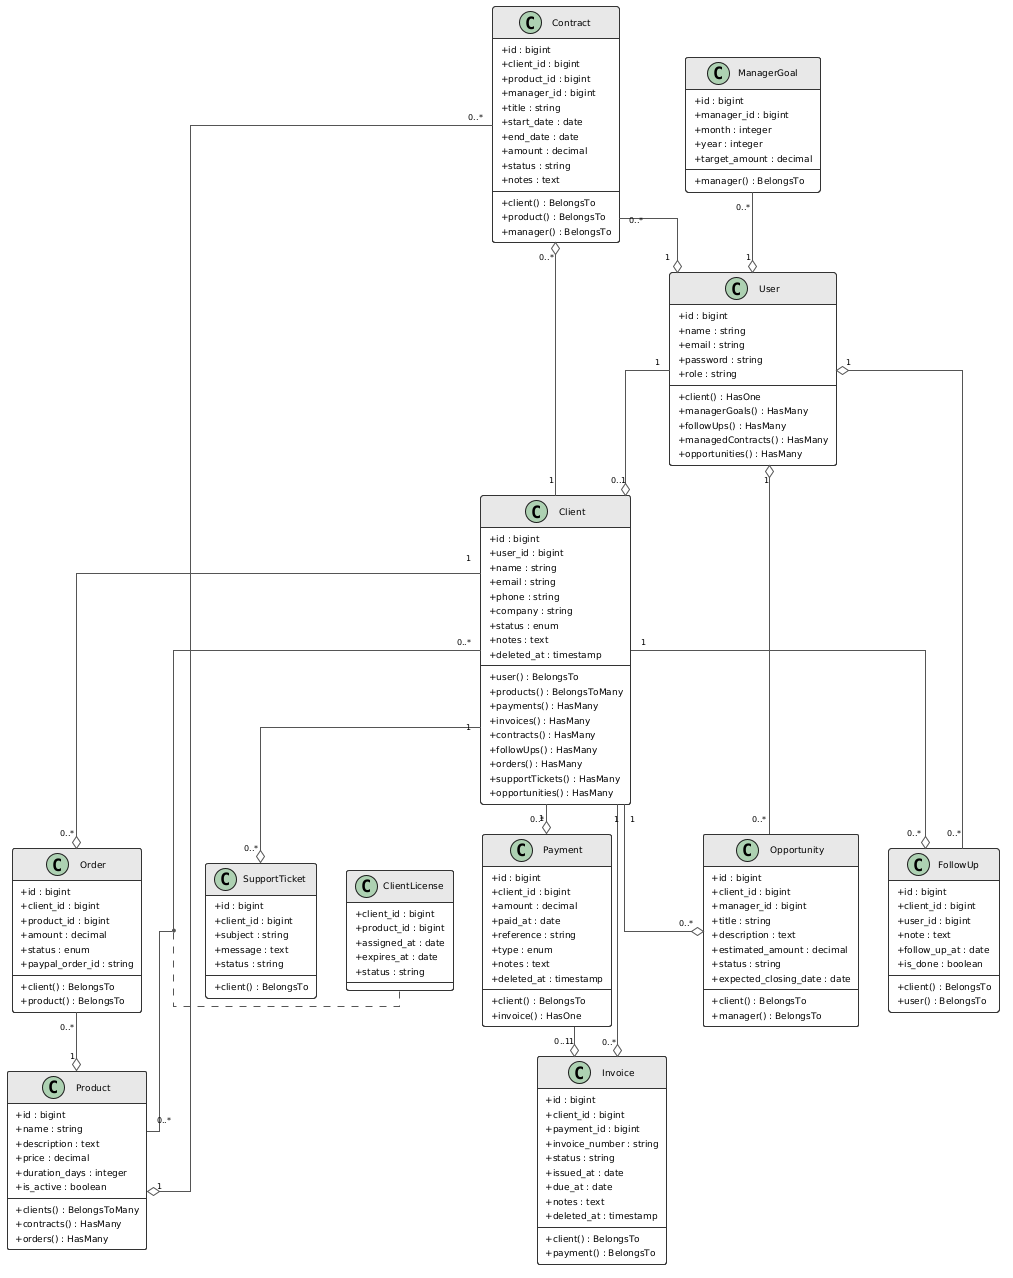
\includegraphics[width=\textwidth]{diagrammes-Classes/diag_classes.png}
  \caption{Diagramme de classes de l'application WAVE}
  \label{fig:classes}
\end{figure}

Le diagramme s'organise autour de deux entites centrales : \textbf{User}
et \textbf{Client}.

La classe \textbf{User} represente tout utilisateur authentifie dans le
systeme, quel que soit son role. Elle stocke les informations d'identite
(nom, email, mot de passe hache) et le champ \texttt{role} qui determine
les droits d'acces. Un User peut avoir une relation HasOne vers un Client
(dans le cas d'un utilisateur client provisionne par le manager), et des
relations HasMany vers les entites ManagerGoal, FollowUp, Contract
(en tant que manager responsable) et Opportunity.

La classe \textbf{Client} est la pierre angulaire de la logique metier.
Elle contient les informations commerciales du client (nom, email, telephone,
societe, statut, notes) et le champ \texttt{deleted\_at} qui permet les
suppressions douces. Un Client est relie a un User via une cle etrangere
\texttt{user\_id} nullable (nullable car un client peut exister sans
compte utilisateur). Il entretient des relations HasMany avec les classes
Payment, Invoice, Contract, FollowUp, Order et SupportTicket. La relation
avec Product est de type ManyToMany via la table pivot
\texttt{client\_license}, qui stocke les dates d'attribution et
d'expiration ainsi que le statut de chaque licence.

La classe \textbf{Product} stocke les informations du catalogue : nom,
description, prix en MAD, duree en jours et le flag \texttt{is\_active}
qui controle la visibilite en boutique. Elle est reliee a Client via la
table pivot \texttt{client\_license}, et a Contract et Order par des
relations BelongsTo.

La classe \textbf{Payment} enregistre chaque transaction financiere avec
son montant, sa date, sa reference et son type via un enum
(\texttt{subscription}, \texttt{license}, \texttt{other}). Elle supporte
les suppressions douces. Elle a une relation HasOne vers Invoice, ce qui
lie automatiquement une facture a son paiement d'origine.

La classe \textbf{Invoice} stocke les factures avec leur numero au format
\texttt{FAC-YYYY-NNNN}, leur statut, leurs dates d'emission et d'echeance.
Elle supporte les suppressions douces et est reliee a Client et Payment
via des cles etrangeres.

La classe \textbf{Contract} modelise les engagements contractuels entre
l'agence et ses clients. Elle reference a la fois le client, le produit
concerne et le manager responsable. Un scope Eloquent
\texttt{expiringWithin} est defini pour filtrer facilement les contrats
expirant dans un delai donne.

Les classes \textbf{Opportunity} et \textbf{FollowUp} couvrent
respectivement le pipeline commercial CRM et les relances commerciales.
Toutes deux referencent un client et un utilisateur manager. FollowUp
dispose d'un champ booleen \texttt{is\_done} pour marquer une relance
comme effectuee.

La classe \textbf{Order} enregistre les commandes passees via PayPal,
avec le champ \texttt{paypal\_order\_id} permettant de faire le lien
avec la transaction PayPal et un enum de statut
(\texttt{pending}, \texttt{completed}, \texttt{cancelled}).

La classe \textbf{SupportTicket} modelise les tickets de support soumis
par les clients, avec leur sujet, leur message et leur statut.

Enfin, la classe \textbf{ManagerGoal} stocke les objectifs mensuels
definis par l'admin pour chaque manager, avec le mois, l'annee et le
montant cible en MAD.

Le tableau \ref{tab:relations} synthetise les principales relations entre
les classes du systeme.

\vspace{0.4cm}
\begin{table}[H]
\centering
\caption{Principales relations Eloquent du systeme}
\label{tab:relations}
\begin{tabularx}{\textwidth}{@{}llX@{}}
\toprule
\textbf{Classe source} & \textbf{Type} & \textbf{Classe cible} \\
\midrule
User          & HasOne      & Client \\[3pt]
User          & HasMany     & ManagerGoal, FollowUp, Contract (manager), Opportunity \\[3pt]
Client        & BelongsTo   & User \\[3pt]
Client        & HasMany     & Payment, Invoice, Contract, FollowUp, Order, SupportTicket \\[3pt]
Client        & BelongsToMany & Product (via client\_license) \\[3pt]
Payment       & HasOne      & Invoice \\[3pt]
Invoice       & BelongsTo   & Client, Payment \\[3pt]
Contract      & BelongsTo   & Client, Product, User (manager) \\[3pt]
Opportunity   & BelongsTo   & Client, User (manager) \\[3pt]
Order         & BelongsTo   & Client, Product \\[3pt]
SupportTicket & BelongsTo   & Client \\[3pt]
ManagerGoal   & BelongsTo   & User (manager) \\
\bottomrule
\end{tabularx}
\end{table}

% ============================================================
\section{Architecture technique}
% ============================================================

\subsection{Architecture API-first}

L'application repose sur une architecture API-first avec une separation
nette entre le backend et le frontend. Le backend est un serveur Laravel
qui expose une API REST sous le prefixe \texttt{/api/v1}. Le frontend
est une Single Page Application React qui consomme cette API via des
requetes HTTP authentifiees. Les deux serveurs fonctionnent de maniere
independante et communiquent exclusivement par echanges JSON.

Cette separation offre plusieurs avantages concrets : le frontend peut
etre deploye sur un hebergeur statique sans dependre de l'infrastructure
PHP, le backend peut etre consomme par d'autres clients (application
mobile, outil tiers) sans modification, et les deux couches peuvent
evoluer independamment l'une de l'autre.

\subsection{Gestion des roles et des acces}

Le controle d'acces est implemente a deux niveaux. Cote backend, le
middleware \texttt{RoleMiddleware} verifie le champ \texttt{role} de
l'utilisateur authentifie avant d'autoriser l'acces a chaque groupe
de routes. Les routes admin sont protegees par
\texttt{middleware(['auth:sanctum', 'role:admin'])},  les routes
back-office par \\ \texttt{role:admin,manager}, 
et les routes espace
client par \texttt{role:client}.

Cote frontend, le composant \texttt{PrivateRoute} inspecte le role
stocke dans le contexte d'authentification et redirige automatiquement
tout utilisateur qui tenterait d'acceder a une section qui ne lui
appartient pas.

\subsection{Gestion asynchrone et taches planifiees}

Les operations longues ou susceptibles d'echouer, notamment l'envoi
d'emails, sont traitees de maniere asynchrone via le systeme de queues
de Laravel. Cela garantit que les actions de l'utilisateur recoivent
une reponse immediate sans attendre la fin de traitements externes.

Les taches recurrentes sont definies dans \texttt{routes/console.php}
et orchestrees par le scheduler Laravel, qui agit comme un cron unifie.
Les trois taches planifiees sont la verification quotidienne des licences
a 08h00, l'envoi des rappels de retard de paiement chaque lundi a 09h00
et la generation du rapport mensuel le premier de chaque mois a 07h00.

% ============================================================
\section{Conclusion}
% ============================================================

Ce deuxieme chapitre a pose les fondations conceptuelles et architecturales
de l'application WAVE. Les diagrammes de cas d'utilisation ont permis de
couvrir exhaustivement l'ensemble des interactions entre les quatre acteurs
du systeme et la plateforme. Les diagrammes de sequence ont mis en lumiere
les flux les plus complexes : la securisation de l'authentification par
token Bearer avec redirection par role, le processus de commande et de
paiement PayPal avec attribution automatique de licence, et le systeme
d'automatisation par taches planifiees pour le suivi des licences.

Le diagramme de classes a revele une architecture de donnees coherente,
organisee autour des entites Client et User, avec des relations Eloquent
bien definies qui facilitent les requetes et garantissent l'integrite
referentielle des donnees.

Ces elements constituent la reference directe qui a guide le developpement
technique. Le chapitre suivant presentera la realisation de l'application :
les choix technologiques justifies, les modules implementes et les
interfaces produites.

\end{document}


